\documentclass[12pt%
%,draft%
,aspectratio=169%
]{beamer}
%
\usepackage{fontspec}
\defaultfontfeatures{Ligatures=TeX}
%\setsansfont{Liberation Sans}
\usepackage{polyglossia}
\setdefaultlanguage{ngerman}
% Alternative template for talks of the Freie Universität Berlin.
% Created by Leonard R. König, <leonard.koenig@fu-berlin.de> following the
% guidelines on www.fu-berlin.de/cd
%
% (c) Leonard König, CC BY 4.0
%
% This template was written against UTF-8 capable LaTeX engines, specifically
% LuaLaTeX.

% Trying to get rather close to the ppt/odp template:
%  http://www.fu-berlin.de/sites/cd/downloads_container/PowerPoint_Praesentation_Anleitung.pdf

%%% font styles
\setbeamerfont{frametitle}{series=\bfseries}
\setbeamerfont{footline}{series=\bfseries}
\setbeamerfont{headline}{series=\bfseries}
\setbeamerfont{alerted text}{series=\bfseries}
%%%

% colordefs
\definecolor{fu_darkblue}{RGB}{0,51,102}
\definecolor{fu_seablue}{RGB}{0,102,204}
\definecolor{fu_lightblue}{RGB}{204,214,224}
\definecolor{fu_green}{RGB}{153,204,0}
\definecolor{fu_lightgrey}{RGB}{128,128,128}
\definecolor{fu_grey}{RGB}{95,95,95}
%
\definecolor{fu_red}{RGB}{204, 0, 0} % red text (used by \alert)
%%% end colordefs

%%% colors
\setbeamercolor*{title}{fg=fu_darkblue}
\setbeamercolor*{subtitle}{fg=fu_seablue}
\setbeamercolor*{frametitle}{fg=fu_darkblue}
\setbeamercolor*{footline}{fg=fu_grey,bg=fu_lightblue}
\setbeamercolor*{headline}{fg=fu_grey}

\setbeamercolor*{normal text}{fg=black}
\setbeamercolor*{alerted text}{fg=fu_red}
\setbeamercolor*{example text}{fg=fu_green}
\setbeamercolor*{structure}{fg=fu_darkblue}

\setbeamercolor*{block title}{fg=white,bg=black!50}
\setbeamercolor*{block title alerted}{fg=white,bg=black!50}
\setbeamercolor*{block title example}{fg=white,bg=black!50}

\setbeamercolor*{block body}{bg=black!10}
\setbeamercolor*{block body alerted}{bg=black!10}
\setbeamercolor*{block body example}{bg=black!10}

\setbeamercolor{bibliography entry author}{fg=fu_darkblue}

\setbeamercolor{item}{fg=fu_darkblue}
\setbeamercolor{navigation symbols}{fg=fu_lightgrey,bg=fu_grey}
%%% end colors

%%% title page
% Display logo (if exists) and right next to it, put our title + subtitle
\defbeamertemplate*{title page}{fu_titlepage}
{%
	\hskip .3\textheight
	\begin{minipage}[.4\textheight]{\textwidth}
		\begin{minipage}[.4\textheight]{0.25\textwidth}
			\inserttitlegraphic
		\end{minipage}%
		\begin{minipage}[.4\textheight]{0.75\textwidth}
			\begin{beamercolorbox}{title}
				\usebeamerfont{title}\inserttitle\par%
			\end{beamercolorbox}
			\vfill
			\ifx\insertsubtitle
				\@empty%
			\else
				\begin{beamercolorbox}{subtitle}
					\usebeamerfont{subtitle}\insertsubtitle\par
				\end{beamercolorbox}
			\fi
		\end{minipage}
	\end{minipage}%
	\hskip .3\textheight
}
%%% end title page

%%% headline
% display title, author and institute on the left;
% logo on the right.
\newcommand{\headlinetext}
{%
	\inserttitle\\[0.3em]%
	\insertauthor, %
	\insertshortinstitute
}
\newlength{\headlinewidth}
\setlength{\headlinewidth}{\paperwidth}
\addtolength{\headlinewidth}{-2\marginparsep}
\setbeamertemplate{headline}
{%
	\begin{beamercolorbox}[wd=\paperwidth]{headline}%
		\vskip5pt
		{\hspace*{\marginparsep}}%
		\parbox{.5\headlinewidth}
		{%
			\usebeamertemplate{title in head/foot}%
			\headlinetext%
		}%
		\begin{minipage}{.5\headlinewidth}%
			\hfill\usebeamertemplate*{logo}
		\end{minipage}%
		{\hspace*{\marginparsep}}%
	\end{beamercolorbox}%
}
%%% end headline

%%% footline
% title + date on the left, frame number on the right
\newcommand{\footlinetext}
{%
	\usebeamerfont{shorttitle}\insertshorttitle, %
	\usebeamerfont{shortdate}\insertshortdate
}
\setbeamertemplate{footline}
{%
	\begin{beamercolorbox}{footline}
		\vskip2pt
		\hspace{\marginparsep}%
		\footlinetext\hfill%
		\insertframenumber%
		\hspace{\marginparsep}
		\vskip2pt
	\end{beamercolorbox}%
}
%%% end footline

% don't use default templates for sidebars
\setbeamertemplate{sidebar right}{}
\setbeamertemplate{sidebar left}{}
\setbeamertemplate{title page}[fu_titlepage]
\usepackage{amsmath}
\usepackage{amsfonts}
\usepackage{amssymb}
\usepackage{graphicx}
\usepackage{algorithm}
\usepackage[noend]{algpseudocode}
%\usepackage{algorithmic}
\usepackage{tikz}
\usetikzlibrary{arrows,shapes,automata,petri,positioning,calc}
\usepackage{graphicx}
\usepackage{subfig}
\usepackage{pgfplots}
\usepackage{venndiagram}
\usepackage{ stmaryrd }
\usepackage{circuitikz}
\usepackage{bohr}
\usepackage{csquotes}


\usepackage{luacode} % for '\luaexec' macro
%% Define a LaTeX "wrapper" macro:
\newcommand\bitwiseXOR[2]{\luaexec{tex.sprint((#1)~(#2))}}
\newcommand\bitwiseAND[2]{\luaexec{tex.sprint((#1)&(#2))}}
\newcommand\bitwiseOR[2]{\luaexec{tex.sprint((#1)|(#2))}}


\def\CalcC#1{%
\coordinate (base) at (#1.B);
\coordinate (collector) at (#1.C);
\coordinate (emitter) at (#1.E);
\draw (barycentric cs:base=0.32,collector=0.5,emitter=0.5) circle [radius=14pt];
}

\pgfplotsset{
    standard/.style={%Axis format configuration
        axis x line=middle,
        axis y line=middle,
        enlarge x limits=0.15,
        enlarge y limits=0.15,
        every axis x label/.style={at={(current axis.right of origin)},anchor=north west},
        every axis y label/.style={at={(current axis.above origin)},anchor=north east},
        every axis plot post/.style={mark options={fill=white}}
        }
    }


\author{Benjamin Tröster}
\title[Schalttechnik \& Logikgatter]{Schalttechnik \& Logikgatter}
%\subtitle[Markov Models]{...}
%\pgfdeclareimage{titlegraphic}{../res/dwarf_logo2.png}
%\titlegraphic{\pgfuseimage{titlegraphic}}
%\date{}
%\subject{}
%
% FU settings
\institute[HTW Berlin]{Hochschule für Technik und Wirtschaft Berlin}
%\pgfdeclareimage[height=0.9cm]{logo}{../res/dwarf_logo}
%\logo{\pgfuseimage{logo}}
%
\usepackage[
backend=biber,
citestyle=alphabetic,bibstyle=authoryear
]{biblatex}
\addbibresource{sources.bib}


\begin{document}

\begin{frame}
\titlepage
\end{frame}

\begin{frame}{Fahrplan}
\tableofcontents[hideothersubsections]
\end{frame}

\section{Wiederholung}

\subsection{Leiter \& Bändermodell}
\begin{frame}{Leiter \& Bändermodell}
\begin{columns}[T] % align columns
\begin{column}{.48\textwidth}
\vspace*{-0.2cm}
\begin{figure}
\center
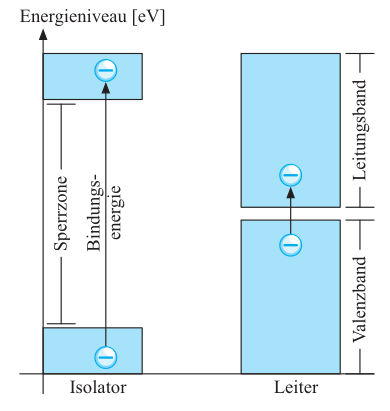
\includegraphics[scale=.45]{pictures/baendermod}
\end{figure}
\end{column}%
\hfill%
\begin{column}{.48\textwidth}
\vspace*{-0.3cm}
\begin{figure}
\center
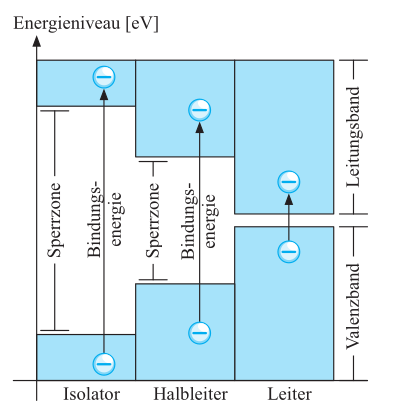
\includegraphics[scale=.45]{pictures/halbleiter_band}
\end{figure}
\end{column}%
\end{columns}
\end{frame}

\begin{frame}
\begin{itemize}
	\item Aufnahme und Abgabe von Energie bestimmt, ob Elektron zwischen Schalen wechseln kann
	\item Elektronen, die z. B. aufgrund thermischer Erhitzung Energie aufnehmen, bewegen sich in Richtung der äußeren Schalen.
	\item Überschreitung des Energieniveau, so verliert das Elektron seine Bindung
	\begin{itemize}
		\item Valenzelektron wird ein freies Leitungselektron
	\end{itemize}
	\item Lösen des Elektron aus Atom $\to$ Bindungsenergie aufgebracht werden
	\item Unterscheidet sich zwischen verschiedenen chemischen Substanzen stark!
	\begin{itemize}
		\item Isolatoren, z. B. Hartgummi sehr hoch
		\item Kupfer/Silber, sehr geringe Energiemenge ausreichend, um freie Leitungselektronen zu erzeugen
	\end{itemize}
\end{itemize}
\end{frame}

\subsection{Reine Halbleiter}
\begin{frame}{Reine Halbleiter}
\begin{itemize}
	\item Spezielle Festkörper: sowohl Isolator wie auch elektrischer Leiter
	\item Eigenschaft aufgrund chemisch/physikalischen Struktur
	\item Bindungsenergie: Material bei geringen Temperaturen zu Isolator 
	\item Aber Bindungsenergie klein genug, um bei mäßigen Temperaturen größeren Anzahl Elektronen überwunden zu werden
	\begin{itemize}
		\item Bsp.: Germanium eine Temperatur von ca. 50 \textdegree C gute elektrische Leitfähigkeit
	\end{itemize}
\end{itemize}
\end{frame}

\begin{frame}{Siliziumgitter}
\begin{columns}[T] % align columns
\begin{column}{.48\textwidth}
\begin{itemize}
	\item Struktur des Siliziumkristalls
	\item Jedes Atom ist von 4 weiteren Atomen umgeben
	\item Jeweils zwei gemeinsam genutzte Valenzelektronen eine stabile Verbindung
\end{itemize}
\end{column}%
\hfill%
\begin{column}{.48\textwidth}
\begin{tikzpicture}[
  baseline=(nucleus.base),
  nucleus options/.style = {draw=black!80,fill=black!10,opacity=.25},
  shell options/.style = {draw=blue!75,thin},
  electron options/.style = {blue!50!black!50},
  silicon/.pic = {
    \node (nucleus) at (0,0) {Si};
    \draw[nucleus options] (nucleus) circle (1em);
    \draw[shell options] (nucleus) circle (2em);
    \foreach \angle in {0,90,180,270} {
      \fill[electron options] (nucleus) ++(\angle:2em) circle (1.5pt);
    }
  },
  ]
  \foreach \angle in {0,90,180,270} {
    \fill[lightgray,rotate=\angle] (2.5em,0) ellipse (1em and .5em);
    \path (\angle:5em) pic {silicon};
  }
  \path (0,0) pic {silicon};
\end{tikzpicture}
\end{column}%
\end{columns}
\end{frame}

\begin{frame}{Eigenleitung im Halbleiterkristall}
\begin{columns}[T] % align columns
\begin{column}{.48\textwidth}
\begin{itemize}
	\item Freigesetzten Leitungselektronen richten sich im elektrischen Feld aus
	\item Freie Elektronen wandern in Richtung der positiven Spannungsquelle
	\item Gleichzeitig entstehende Elektronenlöcher bewegen sich in entgegengesetzter Richtung auf den Minuspol zu
\end{itemize}
\end{column}%
\hfill%
\begin{column}{.48\textwidth}
\vspace*{-0.3cm}
\begin{figure}
\center
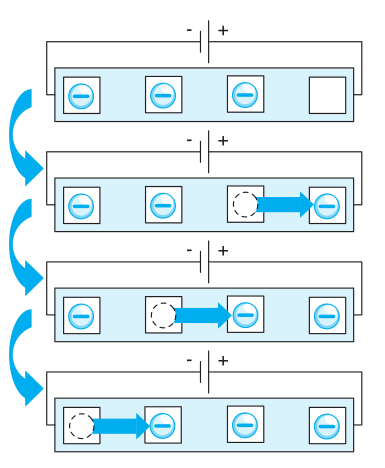
\includegraphics[scale=.4]{pictures/eigenleitung}
\end{figure}
\end{column}%
\end{columns}
\end{frame}


\begin{frame}{Elektronenüberschussleiter: $n$-Leiter}
\begin{columns}[T] % align columns
\begin{column}{.48\textwidth}
\begin{itemize}
	\item Struktur eines Elektronenüberschussleiters ($n$-Leiter)
	\item Einbau von Phosphoratomen zusätzliche Valenzelektronen im Gitter
	\item Zusätzliche Elektronen können sich nahezu ungehindert durch die Kristallstruktur bewegen
\end{itemize}
\end{column}%
\hfill%
\begin{column}{.48\textwidth}
\begin{figure}
\center
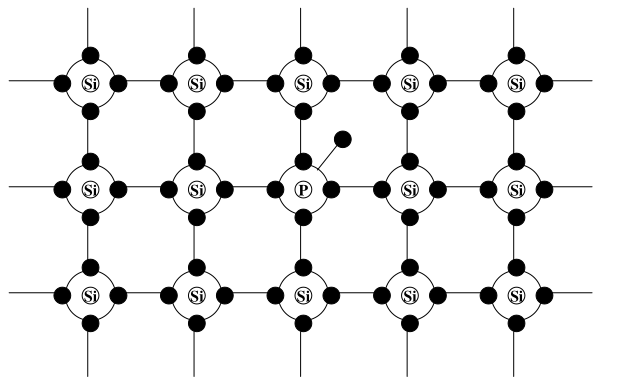
\includegraphics[scale=0.3]{pictures/n_leiter}
\end{figure}
\end{column}%
\end{columns}
\end{frame}

\begin{frame}{Elektronenmangelleiter: $p$-Leiter}
\begin{columns}[T] % align columns
\begin{column}{.48\textwidth}
\begin{itemize}
	\item Struktur eines Elektronenmangelleiters ($p$-Leiter)
	\item Einbau von Aluminiumatomen/Bohr entstehen künstliche Elektronenlöcher
	\item Elektronenlöcher wirken, wie positive Ladungsträger
\end{itemize}
\end{column}%
\hfill%
\begin{column}{.48\textwidth}
\begin{figure}
\center
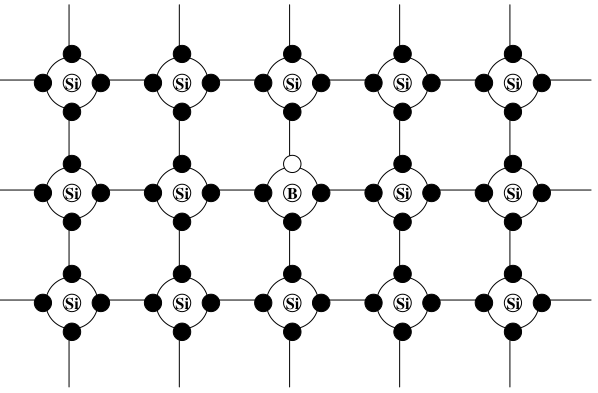
\includegraphics[scale=0.3]{pictures/p_leiter}
\end{figure}
\end{column}%
\end{columns}
\end{frame}

\section{Halbleiter}

\begin{frame}{Leiter/Halbleiter}
	\begin{itemize}
		\item Halbleiter sind Stoffe, deren elektrische Leitfähigkeit geringer als von\\
		Leitern und größer als von Nichtleitern sind
		\item Halbleiter wie Silizium und Germanium verfügen über eine Kristallstruktur
		\item Die Kristallstruktur wird mit hoher Reinheit hergestellt
		\item Auf ca. 1010 Atome kommt ein Fremdatom
		\item Die Eigenleitfähigkeit von Halbleitern basiert auf:
		\begin{itemize}
			\item Verunreinigung
			\item Aufbrechen von Kristallbindungen
			\item Oberflächen-Leitfähigkeit
		\end{itemize}

	\end{itemize}
\end{frame}

\subsection{Halbleiterdioden -- $pn$-Übergang}
\begin{frame}{Halbleiterdioden}
\begin{columns}[T] % align columns
\begin{column}{.48\textwidth}
\begin{itemize}
	\item Dioden: spezielle Schaltelemente
	\item Begrenzung des Stromfluss richtungsabhängig
	\item In Durchlassrichtung neutral
	\item In Sperrrichtung als Isolator
\end{itemize}
\end{column}%
\hfill%
\begin{column}{.48\textwidth}
\begin{figure}
\center
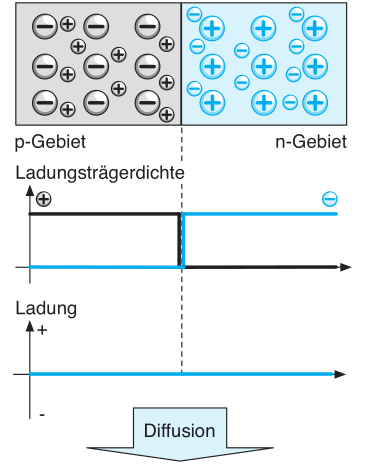
\includegraphics[scale=0.3]{pictures/halbleiterdiode1}
\end{figure}
\end{column}%
\end{columns}
\end{frame}

\begin{frame}{Halbleiterdioden -- $pn$-Übergang}
\begin{columns}[T] % align columns
\begin{column}{.48\textwidth}
\vspace*{0.5cm}
\begin{itemize}
	\item Dioden: spezielle Schaltelemente
	\item Begrenzung des Stromfluss richtungsabhängig
	\item In Durchlassrichtung neutral
	\item In Sperrrichtung als Isolator
\end{itemize}
\end{column}%
\hfill%
\begin{column}{.48\textwidth}
\begin{figure}
\center
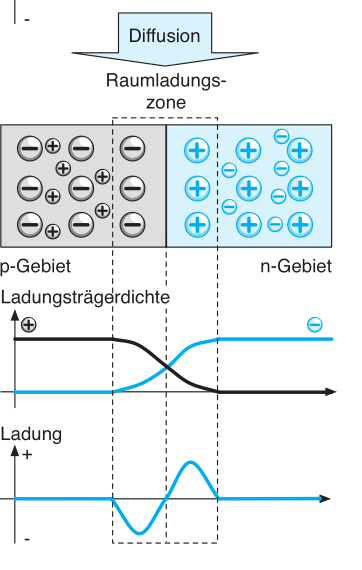
\includegraphics[scale=0.3]{pictures/halbleiterdiode2}
\end{figure}
\end{column}%
\end{columns}
\end{frame}

\begin{frame}{Halbleiterdioden -- $pn$-Übergang}
\begin{columns}[T] % align columns
\begin{column}{.48\textwidth}
\begin{itemize}
	\item Dioden: spezielle Schaltelemente
	\item Begrenzung des Stromfluss richtungsabhängig
	\item In Durchlassrichtung neutral
	\item \textbf{In Sperrrichtung als Isolator}
	\begin{itemize}
		\item Anlegen einer Spannung in Sperrrichtung
		\item Minuspol: $p$-Schicht, Pluspol $n$-Schicht
		\item Ladungsträger Richtung Spannungspole weggezogen
		\item D.h. Vergrößerung Sperrschicht $\to$ Isolator
	\end{itemize}
\end{itemize}
\end{column}%
\hfill%
\begin{column}{.48\textwidth}
\begin{figure}
\center
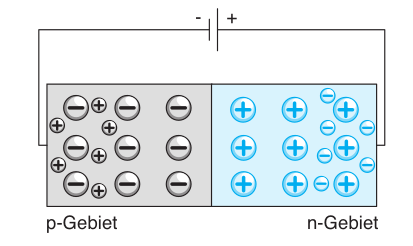
\includegraphics[scale=0.5]{pictures/sperrrichtung}
\end{figure}
\end{column}%
\end{columns}
\end{frame}

\begin{frame}{Halbleiterdioden -- $pn$-Übergang}
\begin{columns}[T] % align columns
\begin{column}{.48\textwidth}
\begin{itemize}
	\item Dioden: spezielle Schaltelemente
	\item Begrenzung des Stromfluss richtungsabhängig
	\item \textbf{In Durchlassrichtung neutral}
	\begin{itemize}
		\item Anlegen einer Spannung in Durchlassrichtung
		\item Pluspol: $p$-Schicht, Minus $p$-Schicht
		\item Freie Ladungsträger bewegen sich aufeinander zu
		\item D.h. Rekombination i.d. Sperrschicht $\to$ Leiter
	\end{itemize}
	\item In Sperrrichtung als Isolator
\end{itemize}
\end{column}%
\hfill%
\begin{column}{.48\textwidth}
\begin{figure}
\center
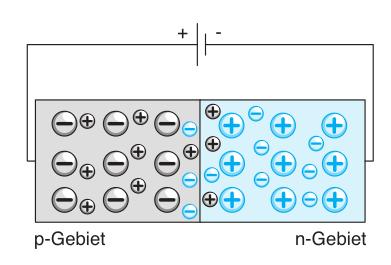
\includegraphics[scale=0.5]{pictures/durchlass}
\end{figure}
\end{column}%
\end{columns}
\end{frame}



\section{Transistor}
\begin{frame}{Transistor -- Transfer Resistor}
\begin{columns}[T] % align columns
\begin{column}{.48\textwidth}
	\begin{itemize}
		\item Gist: steuerbarer Widerstand
		\item Kann elektrisches Signal verstärken
		\item Digital ansteuerbar zum Ein- oder Ausschalten
		\item Bipolare Transistoren
		\begin{itemize}
			\item $npn$-Transistor
			\item $pnp$-Transistor
		\end{itemize}
		\item Unipolare Transistoren -- Feldeffekttransistor
		\begin{itemize}
			\item J-FET
			\item MOS-FET
		\end{itemize}
	\end{itemize}
\end{column}%
\hfill%
\begin{column}{.48\textwidth}
\begin{figure}
\center
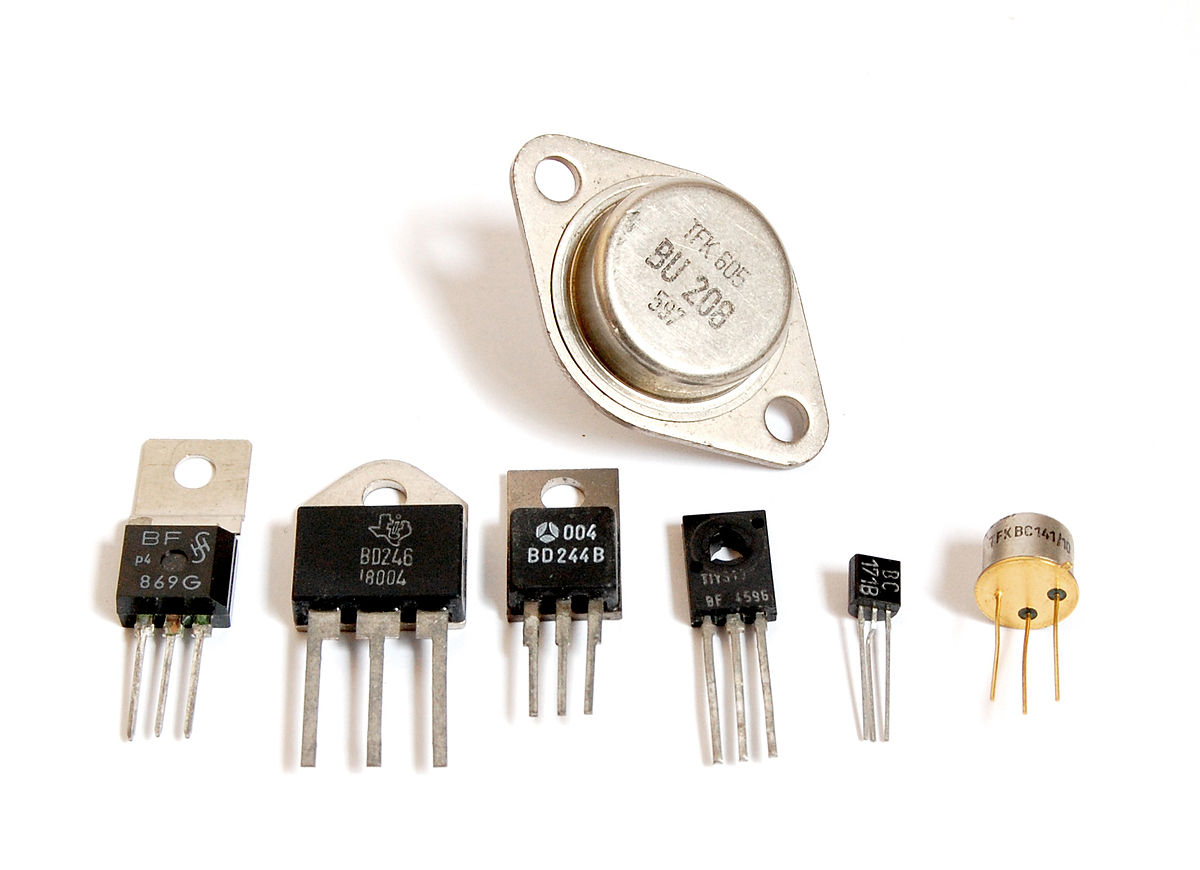
\includegraphics[scale=0.16]{pictures/transistors}
\end{figure}
\end{column}%
\end{columns}
\end{frame}

\subsection{npn-Transistor}
\begin{frame}{$npn$-Transistor}
\begin{columns}[T] % align columns
\begin{column}{.48\textwidth}
	\begin{itemize}
		\item Emitter \& Kollektor dienen Zufluss bzw. Abfluss der Elektronen
		\item Basis: Steueranschluss regelt den Stromfluss zwischen Emitter und Kollektor
		\item Steueranschluss verstärkende Wirkung:
		\begin{itemize}
			\item Geringe Änderung Stromfluss auf Emitter-Basis-Strecke
			\item $\to$ große Änderung des Stromflusses auf Emitter-Kollektor
		\end{itemize}
	\end{itemize}
\end{column}%
\hfill%
\begin{column}{.48\textwidth}
\begin{figure}
\center
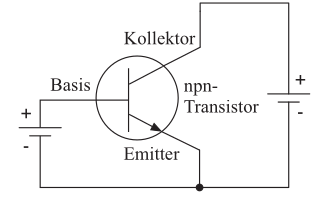
\includegraphics[scale=0.4]{pictures/npn_schema}\\
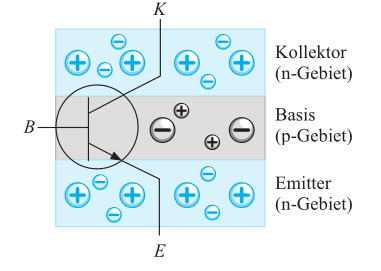
\includegraphics[scale=0.4]{pictures/npn_aufbau}
\end{figure}
\end{column}%
\end{columns}
\end{frame}

\begin{frame}{$npn$-Transistor: Basis-Emitter-Strecke}
\begin{columns}[T] % align columns
\begin{column}{.48\textwidth}
	\begin{itemize}
		\item $pn$-Übergang ist in Durchlassrichtung gepolt
		\item Ermöglicht in Abhängigkeit zur angelegten Spannung einen Stromfluss im Basisstromkreis
	\end{itemize}
\end{column}%
\hfill%
\begin{column}{.48\textwidth}
\begin{figure}
\center
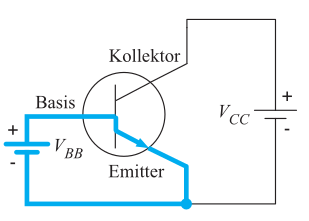
\includegraphics[scale=0.6]{pictures/be}
\end{figure}
\end{column}%
\end{columns}
\end{frame}

\begin{frame}{$npn$-Transistor: Basis-Kollektor-Strecke}
\begin{columns}[T] % align columns
\begin{column}{.48\textwidth}
	\begin{itemize}
		\item Basis besitzt gegenüber Kollektor negatives elektrisches Potenzial
		\item Stromfluss wird durch den in Sperrichtung gepolten $pn$-Übergang unterbunden
	\end{itemize}
\end{column}%
\hfill%
\begin{column}{.48\textwidth}
\begin{figure}
\center
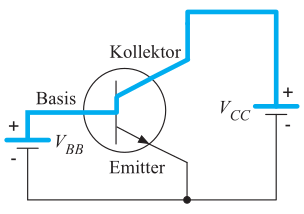
\includegraphics[scale=0.6]{pictures/bk}
\end{figure}
\end{column}%
\end{columns}
\end{frame}

\begin{frame}{$npn$-Transistor: Emitter-Kollektor-Strecke}
\begin{columns}[T] % align columns
\begin{column}{.48\textwidth}
	\begin{itemize}
		\item Zwischen Emitter und Kollektor stellt sich ein Stromfluss ein
		\item Stärke proportional mit der Stärke des Basisstroms zunimmt
	\end{itemize}
\end{column}%
\hfill%
\begin{column}{.48\textwidth}
\begin{figure}
\center
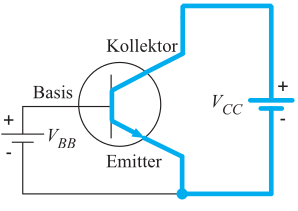
\includegraphics[scale=0.6]{pictures/ek}
\end{figure}
\end{column}%
\end{columns}
\end{frame}

\begin{frame}{$pnp$-Transistor: Emitter-Kollektor-Strecke}
\begin{columns}[T] % align columns
\begin{column}{.58\textwidth}
	\begin{itemize}
		\item Zusammensetzung der Halbleiter \enquote{invers} zu $pnp$
		\item Basis $n$-Gebiet
		\item Emitter und Kollektor dagegen $p$-Gebiet
		\item Positive Spannung am Emitter eine Flut von Elektronenlöchern aus dem $p$-Leiter in das $n$-Gebie
		\item Negative Spannung	: fließt geringer Teil der Defektelektronen über Basis ab
		\item Großteil der Elektronenlöcher wird durch die starke negative Kollektorspannung in die obere $p$-Schicht gezogen
		\item $\to$ fließt als Kollektorenstrom ab
	\end{itemize}
\end{column}%
\hfill%
\begin{column}{.38\textwidth}
\begin{figure}
\center
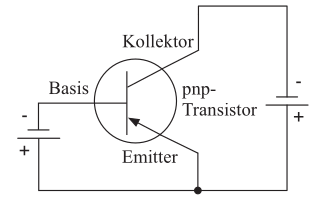
\includegraphics[scale=0.4]{pictures/pnp_schema}\\
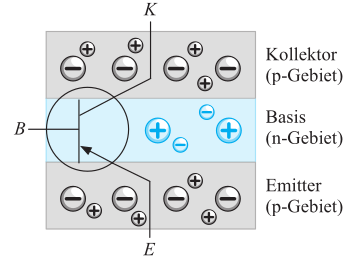
\includegraphics[scale=0.4]{pictures/pnp_aufbau}
\end{figure}
\end{column}%
\end{columns}
\end{frame}

\subsection{Schaltungen mit npn-Transistor}
\begin{frame}{Buffer-Schaltungen mit $npn$-Transistor}
\begin{figure}
\center
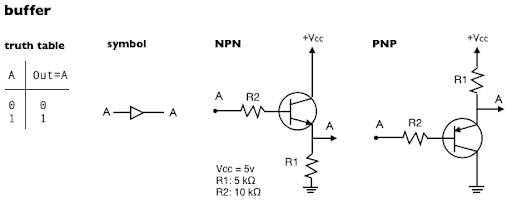
\includegraphics[scale=0.8]{pictures/buffer}
\end{figure}
\end{frame}


\begin{frame}{Not-Schaltungen mit $npn$-Transistor}
\begin{figure}
\center
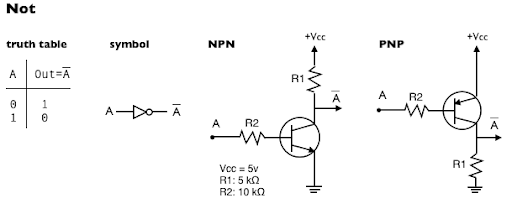
\includegraphics[scale=0.8]{pictures/not}
\end{figure}
\end{frame}


\begin{frame}{AND-Schaltungen mit $npn$-Transistor}
\begin{figure}
\center
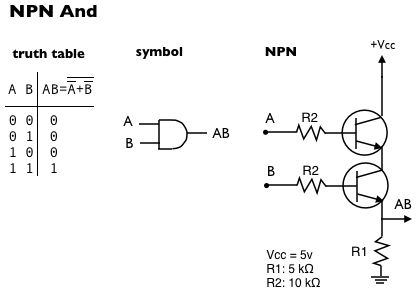
\includegraphics[scale=0.65]{pictures/and}
\end{figure}
\end{frame}

\begin{frame}{NAND-Schaltungen mit $npn$-Transistor}
\begin{figure}
\center
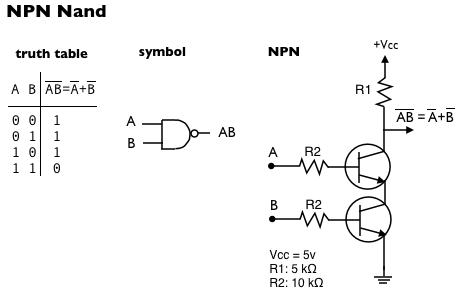
\includegraphics[scale=0.65]{pictures/nand}
\end{figure}
\end{frame}


\begin{frame}{OR-Schaltungen mit $npn$-Transistor}
\begin{figure}
\center
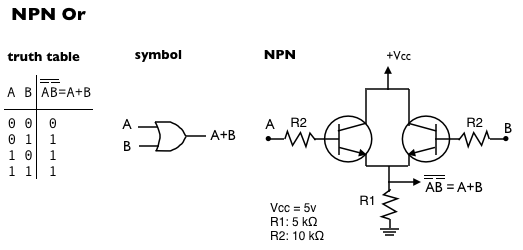
\includegraphics[scale=0.6]{pictures/or}
\end{figure}
\end{frame}

\begin{frame}{NOR-Schaltungen mit $npn$-Transistor}
\begin{figure}
\center
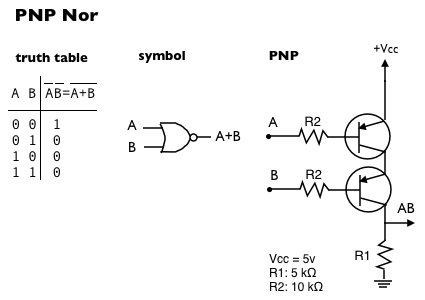
\includegraphics[scale=0.65]{pictures/nor}
\end{figure}
\end{frame}

\subsection{Feldeffekttransistoren}
\begin{frame}{Feldeffekttransistoren: JFET}
\begin{columns}[T] % align columns
\begin{column}{.58\textwidth}
	\begin{itemize}
		\item Funktional Äquivalent
		\item Gate-Anschluss JFET entspricht der Basis
		\item Drain-Anschluss ist der Kollektor
		\item Source-Anschluss dem Emitter
	\end{itemize}
\end{column}%
\hfill%
\begin{column}{.38\textwidth}
\begin{figure}
\center
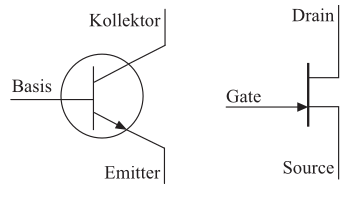
\includegraphics[scale=0.4]{pictures/npn_jfet}\\
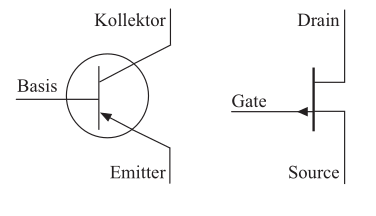
\includegraphics[scale=0.4]{pictures/pnp_jfet}
\end{figure}
\end{column}%
\end{columns}
\end{frame}

\begin{frame}{Feldeffekttransistoren: JFET}
\begin{columns}[T] % align columns
\begin{column}{.58\textwidth}
	\begin{itemize}
		\item Source und Drain sind durch dotierten Halbleiterkanal verbunden
		\item Mitte durch zwei komplementär dotierte Gebiete -- dem Gate
		\item Kanal $n$-dotiert und das Gate $p$-dotiert
		\begin{itemize}
			\item $n$-Kanal-JFET
		\end{itemize}
		\item Kanal $p$-dotierten und $n$ dotierten Gate-Gebiet
		\begin{itemize}
			\item $p$-Kanal-JFET
		\end{itemize}
	\end{itemize}
\end{column}%
\hfill%
\begin{column}{.38\textwidth}
\begin{figure}
\center
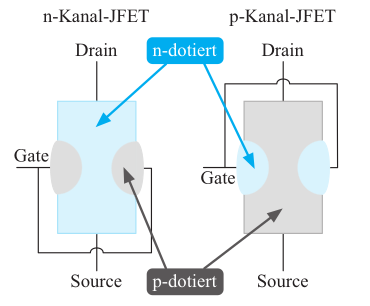
\includegraphics[scale=0.4]{pictures/jfet_aufbau}\\
\end{figure}
\end{column}%
\end{columns}
\end{frame}

\begin{frame}{$n$-Kanal-JFET}
\begin{figure}
\center
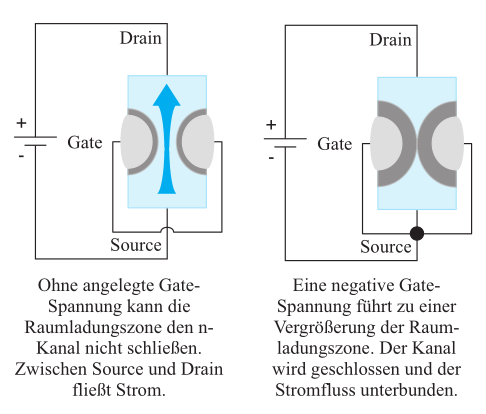
\includegraphics[scale=0.4]{pictures/n_jfet}
\end{figure}
\end{frame}

\begin{frame}{$p$-Kanal-JFET}
\begin{figure}
\center
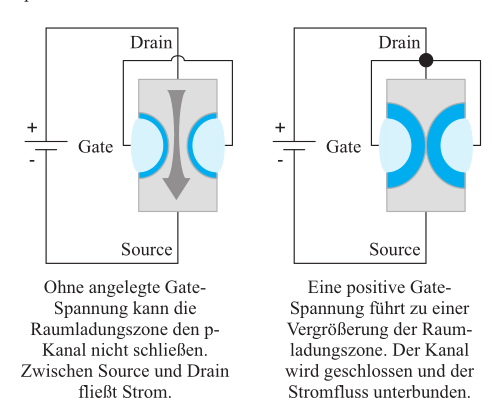
\includegraphics[scale=0.4]{pictures/p_jfet}
\end{figure}
\end{frame}

\subsection{MOS-Feldeffekttransistoren}
\begin{frame}{MOS-Feldeffekttransistoren (MOSFETs)}
\begin{columns}[T] % align columns
\begin{column}{.58\textwidth}
	\begin{itemize}
		\item MOS-Technik (MOS = Metal Oxide Semiconductor)
		\item Funktional entspricht MOSFET weitgehend dem JFET
		\begin{itemize}
			\item Stromfluss zwischen Source- \& Drain-Anschluss, Gate angelegtes elektrisches Feld beeinflusst
			\item Wieder zwei Varianten: $p$ und $n$		
		\end{itemize}
	\end{itemize}
\end{column}%
\hfill%
\begin{column}{.38\textwidth}
\begin{figure}
\center
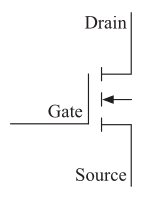
\includegraphics[scale=0.4]{pictures/n_mosfet}\\
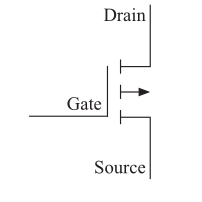
\includegraphics[scale=0.4]{pictures/p_mosfet}
\end{figure}
\end{column}%
\end{columns}
\end{frame}

\begin{frame}{MOS-Feldeffekttransistoren (MOSFETs)}
\begin{columns}[T] % align columns
\begin{column}{.58\textwidth}
	\begin{itemize}
		\item $p$-dotierten Substrat
		\item Drain- und Source-Anschlüsse auf $n$-dotierter Gebiete
		\item Dazwischen Gate, das als dünne Metall- oder Polysiliziumschicht auf Substratoberfläche
		\item Gate und Substrat isolierendes Dielektrikum voneinander getrennt
		\begin{itemize}
			\item Wirkt, wie kleiner Kondensator (speichert also die elektrische Ladung)
		\end{itemize}
	\end{itemize}
\end{column}%
\hfill%
\begin{column}{.38\textwidth}
\begin{figure}
\center
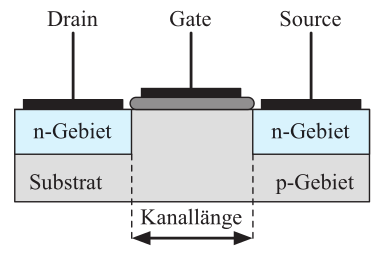
\includegraphics[scale=0.4]{pictures/intern_mosfet}
\end{figure}
\end{column}%
\end{columns}
\end{frame}

\begin{frame}{$n$-MOS-Feldeffekttransistoren}
\begin{itemize}
	\item $V_{DS}$ die Spannung Drain-Source-Strecke
	\item $V_{GS}$ die Spannung Gate-Source-Strecke
	\item Source-Anschluss und das Substrat das gleiche elektrische Potenzial
	\begin{itemize}
		\item $V_{GS}$ gleichermaßen die Spannung zwischen Gate \& Substrat.
	\end{itemize}
\end{itemize}
\end{frame}

\begin{frame}{$V_{GS} = 0$}
\begin{columns}[T] % align columns
\begin{column}{.62\textwidth}
	\begin{itemize}
		\item Drain, Substrat und Source operieren als klassischer $npn$-Übergang
		\item Halbleiterkristall verhält sich wie entgegengesetzte Dioden
		\item D.h. Stromfluss in beide Richtungen unterbrochen
		\item Drain- an Pluspol \& Source-Anschluss Minuspol, so sperrt der linke $pn$-Übergang
		\item Durch Umpolen der Spannung in Durchlassrichtung geschaltet
		\begin{itemize}
			\item Rechter Übergang in den sperrenden Zustand, verhindert den Ladungstransport
		\end{itemize}
	\end{itemize}
\end{column}%
\hfill%
\begin{column}{.38\textwidth}
\begin{figure}
\center
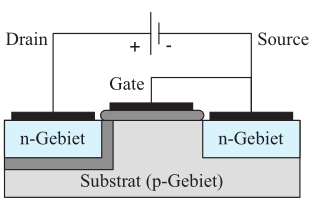
\includegraphics[scale=0.5]{pictures/fall1}\\
\end{figure}
\end{column}%
\end{columns}
\end{frame}

\begin{frame}{$V_{GS} > 0, V_{DS} = 0$}
\begin{columns}[T] % align columns
\begin{column}{.62\textwidth}
	\begin{itemize}
		\item Positive Spannung gegenüber dem Source-Anschluss
		\item Minoritätsträger -- $p$-dotierten Substrats die Elektronen, nach oben gezogen
		\item Grenzschicht zwischen Dielektrium und Substrat rekombinieren mit Elektronenlöchern
		\item Führt zur Verarmung der Majoritätsträger
		\item Überschreitet die Spannung Schwellwert,
		\begin{itemize}
			\item Mehr Elektronen in Grenzschicht gezogen,
			\item als für eine vollständige Rekombination gebraucht werden
		\end{itemize}
		\item Kleiner, leitender $n$-Kanal entsteht
		\item Höhere Spannung $\to$ höherer Durchfluss
	\end{itemize}
\end{column}%
\hfill%
\begin{column}{.38\textwidth}
\begin{figure}
\center
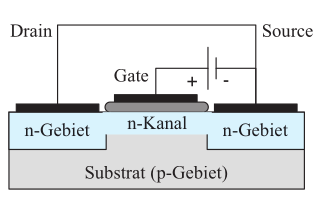
\includegraphics[scale=0.5]{pictures/fall2}\\
\end{figure}
\end{column}%
\end{columns}
\end{frame}

\begin{frame}{$V_{GS} > 0, V_{DS} > 0$}
\begin{columns}[T] % align columns
\begin{column}{.62\textwidth}
	\begin{itemize}
		\item Anlegen der Spannung Gate \& Source $\to$ leitende Inversionszone
		\item Spannung zwischen den beiden Anschlüssen: fließt Strom im geöffneten Kanal
		\item Verengung der Inversionszone durch die entstehenden elektrischen Felder Richtung des Drain-Anschlusses
		\item Ab gewisser Spannung: freien Ladungsträgern können nicht mehr passieren
		\item Sukzessive Erhöhung Spannung Drain-Source-Strecke ab Wert keiner weiteren Erhöhung des Stromflusses führt
	\end{itemize}
\end{column}%
\hfill%
\begin{column}{.38\textwidth}
\begin{figure}
\center
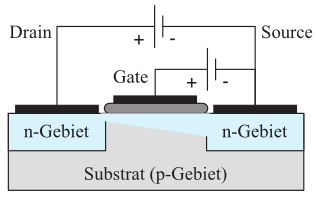
\includegraphics[scale=0.5]{pictures/fall3}\\
\end{figure}
\end{column}%
\end{columns}
\end{frame}


\section*{Quellen}
\appendix
\begin{frame}[allowframebreaks]
  \frametitle<presentation>{Quellen}
\printbibliography
\end{frame}
\end{document}